%% arrowLength=4
%% linkWidth=5
%% input fy=100*node.pos
%% output fx=400
%% output fy=100*node.pos+50
%% MAX_FONT_SIZE=8
\begin{table}[H]
    \begin{center}
        \begin{tabular}{||l c c c||}
            \hline
            & 1      & 2      & 3 \\ [0.5ex]
            \hline
            velikost populacije               & 100    & 150    & 200    \\
            \hline
            največje število globokih vozlišč & 5      & 10     & 15     \\
            \hline
            največje število povezav          & 10     & 20     & 30     \\
            \hline
            največje število prečkanj         & 2      & 2      & 3      \\
            \hline
            delež mutiranih potomcev          & 10\%   & 10\%   & 10\%   \\
            \hline
            prispevek vozlišč                 & -0.001 & -0.001 & -0.001 \\
            \hline
            prispevek povezav                 & -0.001 & -0.001 & -0.001 \\
            \hline
            število generacij                 & 200    & 200    & 300    \\
            \hline
        \end{tabular}
    \end{center}
    \caption{Nabori inicializacijskih parametrov poganjanja na množici Iris.}
    \label{tab:param_iris}
\end{table}

\subsection{Prvi nabor}\label{subsec:dodatek-iris-prvi-nabor}
%%"/home/jure/CLionProjects/Neuroevolution/datasets/iris/iris.data" 100 5 10 2 true 0.1 50 true -0.001 -0.001 200 ACC
\begin{table}[H]
    \begin{center}
        \begin{tabular}{|| c | c c || c c ||}
            \hline
            \multirow{2}{*}{št. zagona} & \multicolumn{2}{c||}{točnost najboljšega agenta} & \multicolumn{2}{c||}{MCC najboljšega agenta} \\ \cline{2-5}
            & učna    & testna           & učna  & testna         \\
            \hline
            1        & 96.2\% & \textbf{93.3\%} & 0.612 & 0.612          \\
            \hline
            2        & 94.3\% & 93.3\%          & 0.612 & 0.612          \\
            \hline
            3        & 90.5\% & 88.9\%          & 0.667 & 0.609          \\
            \hline
            4        & 66.7\% & 66.7\%          & 0.849 & \textbf{0.871 (91.1\%)} \\
            \hline
            5        & 95.2\% & 91.1\%          & 0.612 & 0.552          \\
            \hline
            $\sigma$ & 0.111   & 0.101            & 0.092 & 0.112          \\
            \hline
        \end{tabular}
    \end{center}
    \caption{Rezultat prvega nabora parametrov.}
    \label{tab:iris_result_1}
\end{table}

\begin{table}[H]
    \centering
    \begin{tabular}{||rcccc||}
        \hline
        razred           & Iris Setosa & Iris Versicolour & Iris Virginica & vsota \\ \hline
        Iris Setosa      & 15          & 0                & 0              & 15    \\ \hline
        Iris Versicolour & 0           & 13               & 2              & 15    \\ \hline
        Iris Virginica   & 0           & 1                & 14             & 15    \\ \hline
        vsota            & 15          & 14               & 16             & 45    \\ \hline
    \end{tabular}
    \caption{Matrika zmot najbolj točnega agenta prvega nabora.}
    \label{tab:iris_acc_1}
\end{table}

\begin{table}[H]
    \centering
    \begin{tabular}{||rcccc||}
        \hline
        razred           & Iris Setosa & Iris Versicolour & Iris Virginica & vsota \\ \hline
        Iris Setosa      & 15          & 0                & 0              & 15    \\ \hline
        Iris Versicolour & 1           & 14               & 0              & 15    \\ \hline
        Iris Virginica   & 0           & 3                & 12             & 15    \\ \hline
        vsota            & 16          & 17               & 12             & 45    \\ \hline
    \end{tabular}
    \caption{Matrika zmot agenta z največjim MCC prvega nabora.}
    \label{tab:iris_mcc_1}
\end{table}

\begin{figure}[H]
    \begin{center}
        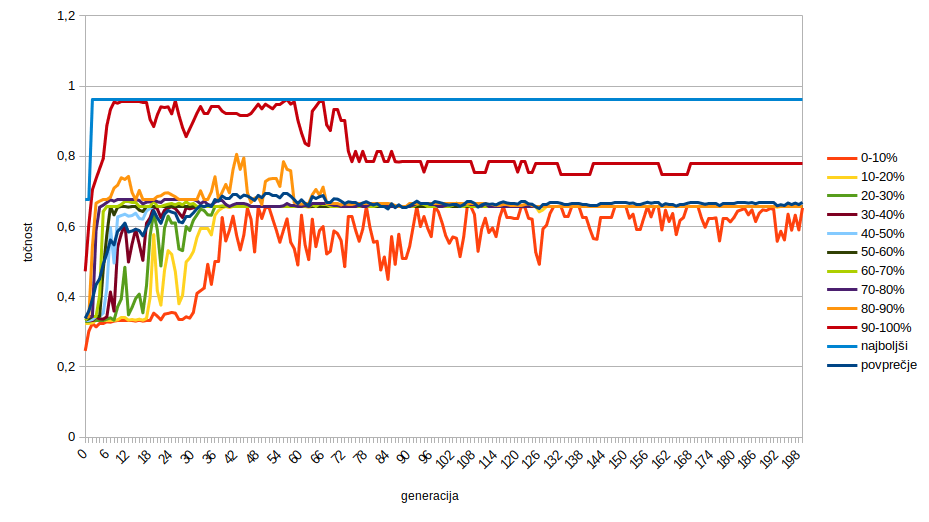
\includegraphics[width=13cm]{iris/1/acc}
    \end{center}
    \caption{Graf točnosti populacije najboljšega agenta prvega nabora skozi generacije.}
    \label{fig:iris_acc_1}
\end{figure}

\begin{figure}[H]
    \begin{center}
        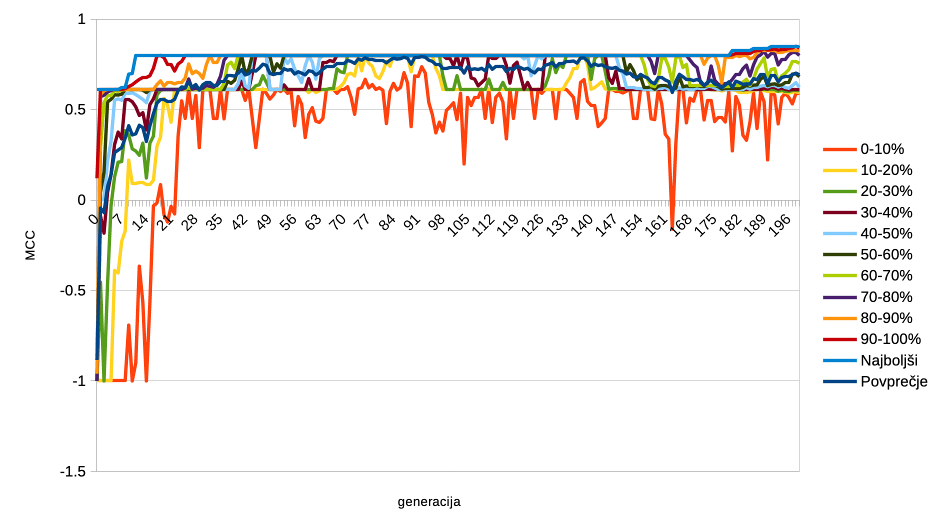
\includegraphics[width=13cm]{iris/1/mcc}
    \end{center}
    \caption{Graf MCC populacije najboljšega agenta prvega nabora skozi generacije.}
    \label{fig:iris_mcc_1}
\end{figure}

\begin{figure}[H]
    \begin{center}
        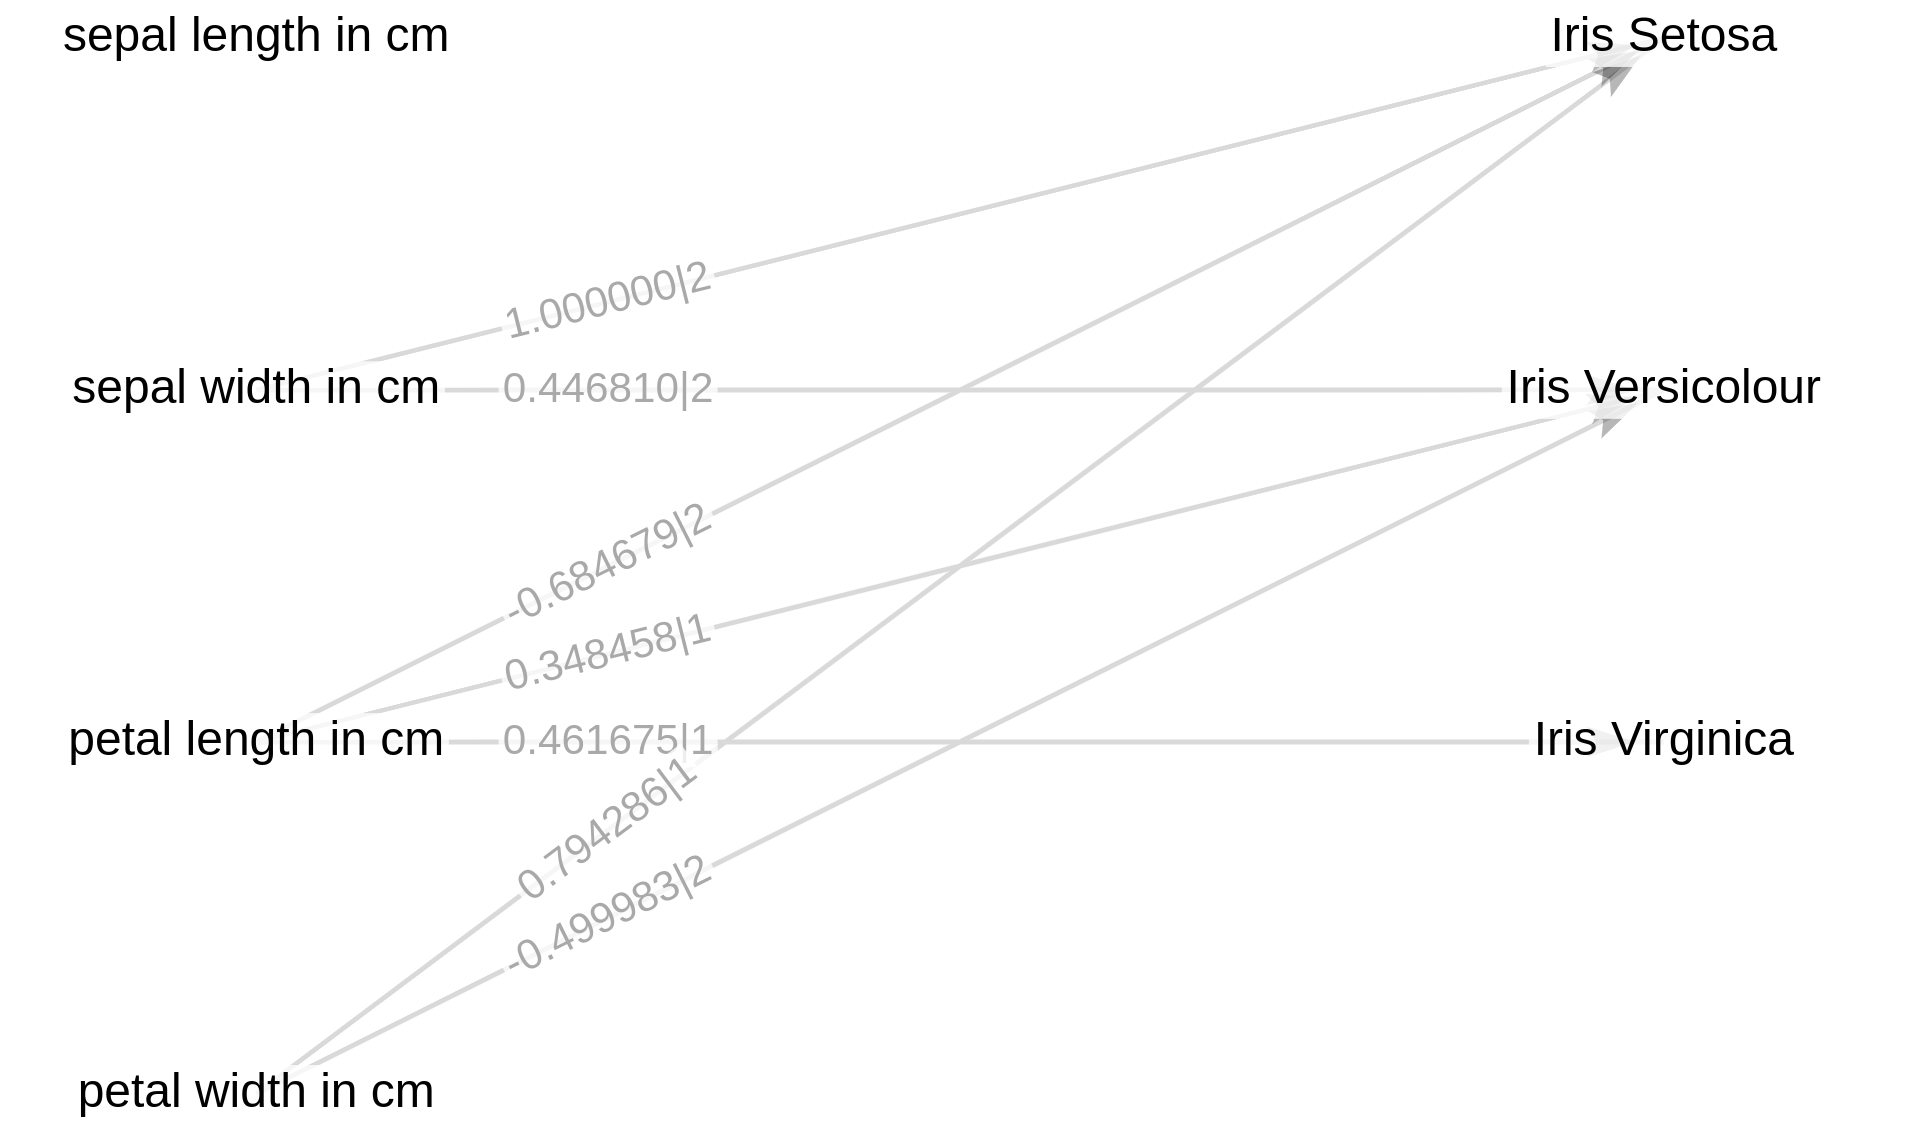
\includegraphics[width=13cm]{iris/1/acc_g}
    \end{center}
    \caption{Vizualizacija najbolj točnega agenta prvega nabora. Vsebuje 5 povezav.}
    \label{fig:iris_acc_1_g}
\end{figure}

\begin{figure}[H]
    \begin{center}
        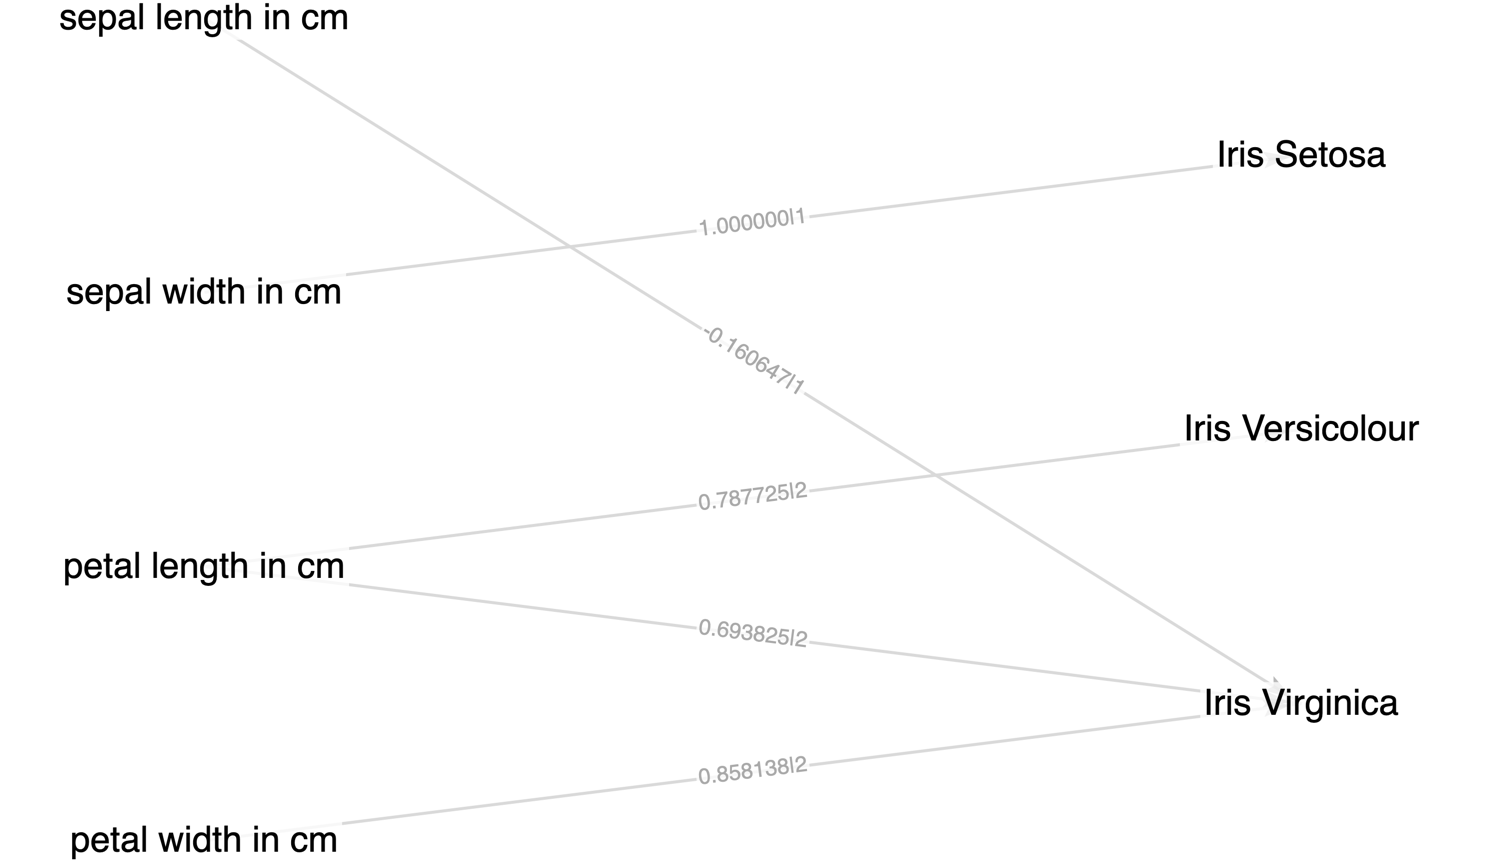
\includegraphics[width=13cm]{iris/1/mcc_g}
    \end{center}
    \caption{Vizualizacija agenta z največjim MCC prvega nabora. Vsebuje 5 povezav.}
    \label{fig:iris_mcc_1_g}
\end{figure}

\subsection{Drugi nabor}\label{subsec:dodatek-iris-drugi-nabor}
%%"/home/jure/CLionProjects/Neuroevolution/datasets/iris/iris.data" 150 10 20 2 true 0.1 75 true -0.001 -0.001 200 ACC
\begin{table}[H]
    \begin{center}
        \begin{tabular}{|| c | c c || c c ||}
            \hline
            \multirow{2}{*}{št. zagona} & \multicolumn{2}{c||}{točnost najboljšega agenta} & \multicolumn{2}{c||}{MCC najboljšega agenta} \\ \cline{2-5}
            & učna    & testna           & učna  & testna         \\
            \hline
            1        & 94.3\% & 95.6\%          & 0.957 & 0.906          \\
            \hline
            2        & 97.1\% & \textbf{97.8\%} & 0.957 & 0.901          \\
            \hline
            3        & 97.1\% & 91.1\%          & 0.929 & 0.877          \\
            \hline
            4        & 93.3\% & 97.8\%          & 0.972 & 0.906          \\
            \hline
            5        & 84.8\% & 88.9\%          & 0.958 & \textbf{1.000 (100\%)} \\
            \hline
            $\sigma$ & 0.045   & 0.036            & 0.014 & 0.042          \\
            \hline
        \end{tabular}
    \end{center}
    \caption{Rezultat drugega nabora parametrov.}
    \label{tab:iris_result_2}
\end{table}

\begin{table}[H]
    \centering
    \begin{tabular}{||rcccc||}
        \hline
        razred           & Iris Setosa & Iris Versicolour & Iris Virginica & vsota \\ \hline
        ris Setosa       & 15          & 0                & 0              & 15    \\ \hline
        Iris Versicolour & 0           & 15               & 0              & 15    \\ \hline
        Iris Virginica   & 0           & 1                & 14             & 15    \\ \hline
        vsota            & 15          & 16               & 14             & 45    \\ \hline
    \end{tabular}
    \caption{Matrika zmot najbolj točnega agenta drugega nabora.}
    \label{tab:iris_acc_2}
\end{table}

\begin{table}[H]
    \centering
    \begin{tabular}{||rcccc||}
        \hline
        razred           & Iris Setosa & Iris Versicolour & Iris Virginica & vsota \\ \hline
        ris Setosa       & 15          & 0                & 0              & 15    \\ \hline
        Iris Versicolour & 0           & 15               & 0              & 15    \\ \hline
        Iris Virginica   & 0           & 0                & 15             & 15    \\ \hline
        vsota            & 15          & 15               & 15             & 45    \\ \hline
    \end{tabular}
    \caption{Matrika zmot agenta z največjim MCC drugega nabora.}
    \label{tab:iris_mcc_2}
\end{table}

\begin{figure}[H]
    \begin{center}
        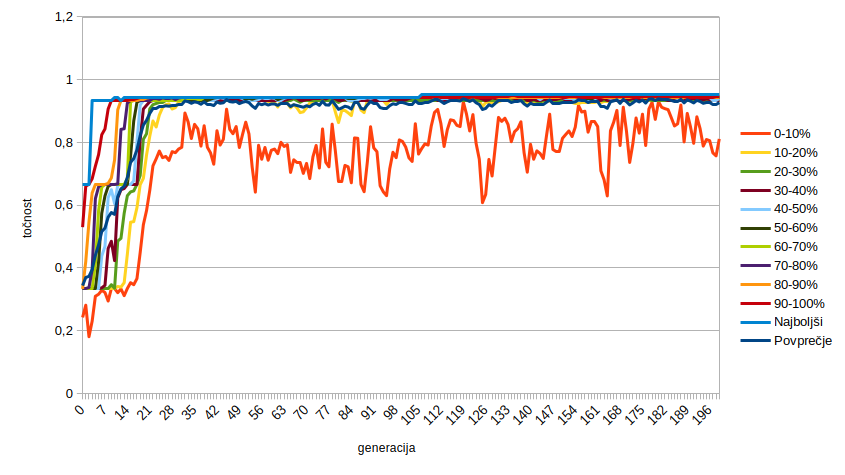
\includegraphics[width=13cm]{iris/2/acc}
    \end{center}
    \caption{Graf točnosti populacije najboljšega agenta drugega nabora skozi generacije.}
    \label{fig:iris_acc_2}
\end{figure}

\begin{figure}[H]
    \begin{center}
        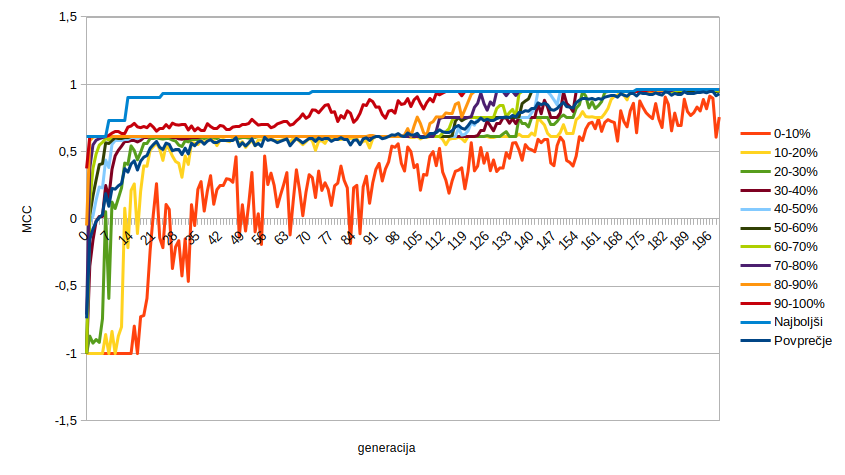
\includegraphics[width=13cm]{iris/2/mcc}
    \end{center}
    \caption{Graf MCC populacije najboljšega agenta drugega nabora skozi generacije.}
    \label{fig:iris_mcc_2}
\end{figure}

\begin{figure}[H]
    \begin{center}
        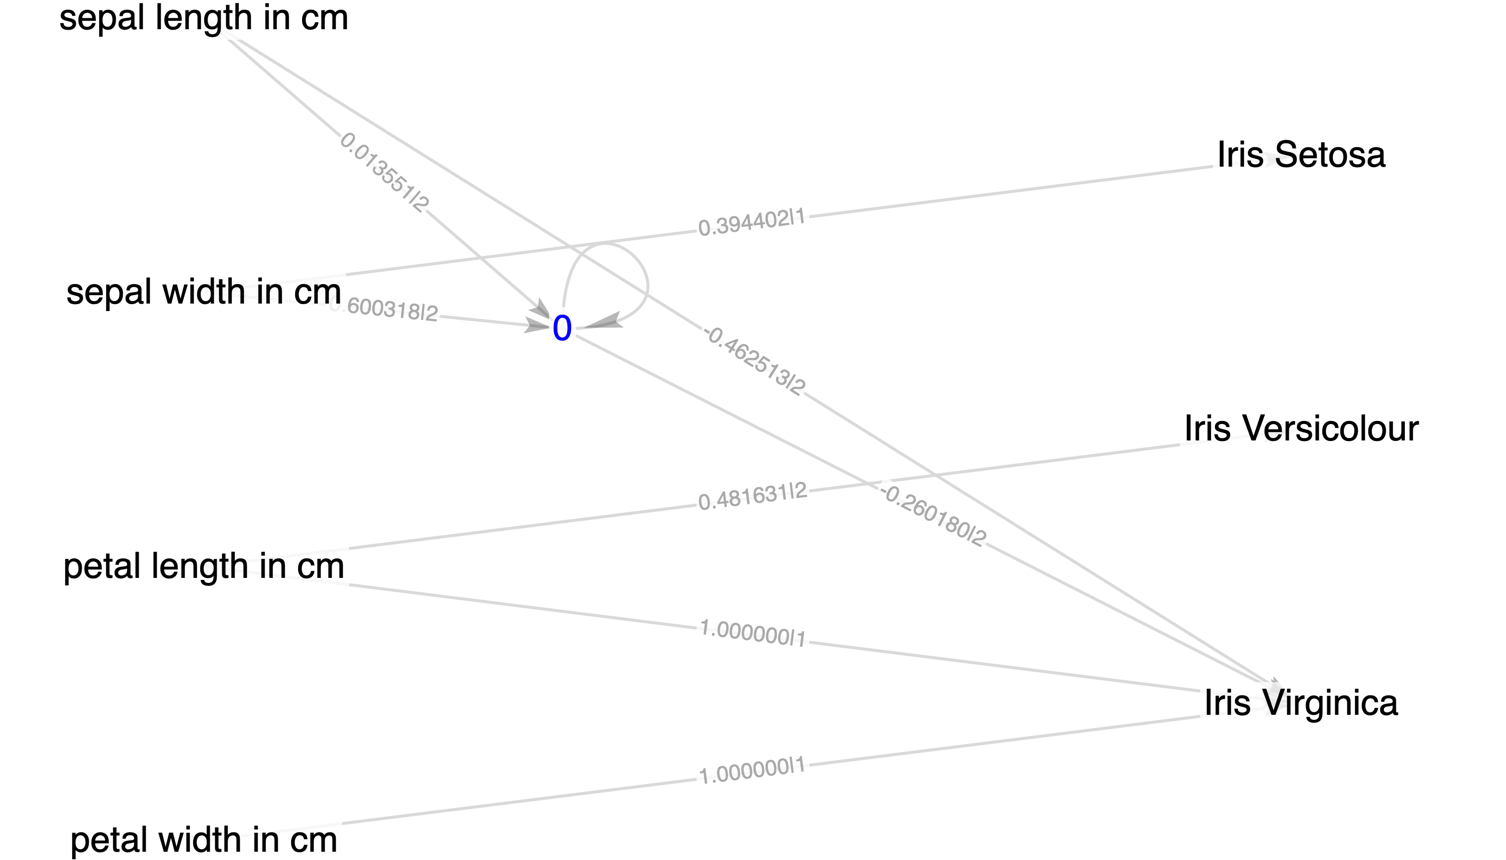
\includegraphics[width=13cm]{iris/2/acc_g}
    \end{center}
    \caption{Vizualizacija najbolj točnega agenta drugega nabora. Vsebuje 1 globoko vozlišče in 9 povezav.}
    \label{fig:iris_acc_2_g}
\end{figure}

\begin{figure}[H]
    \begin{center}
        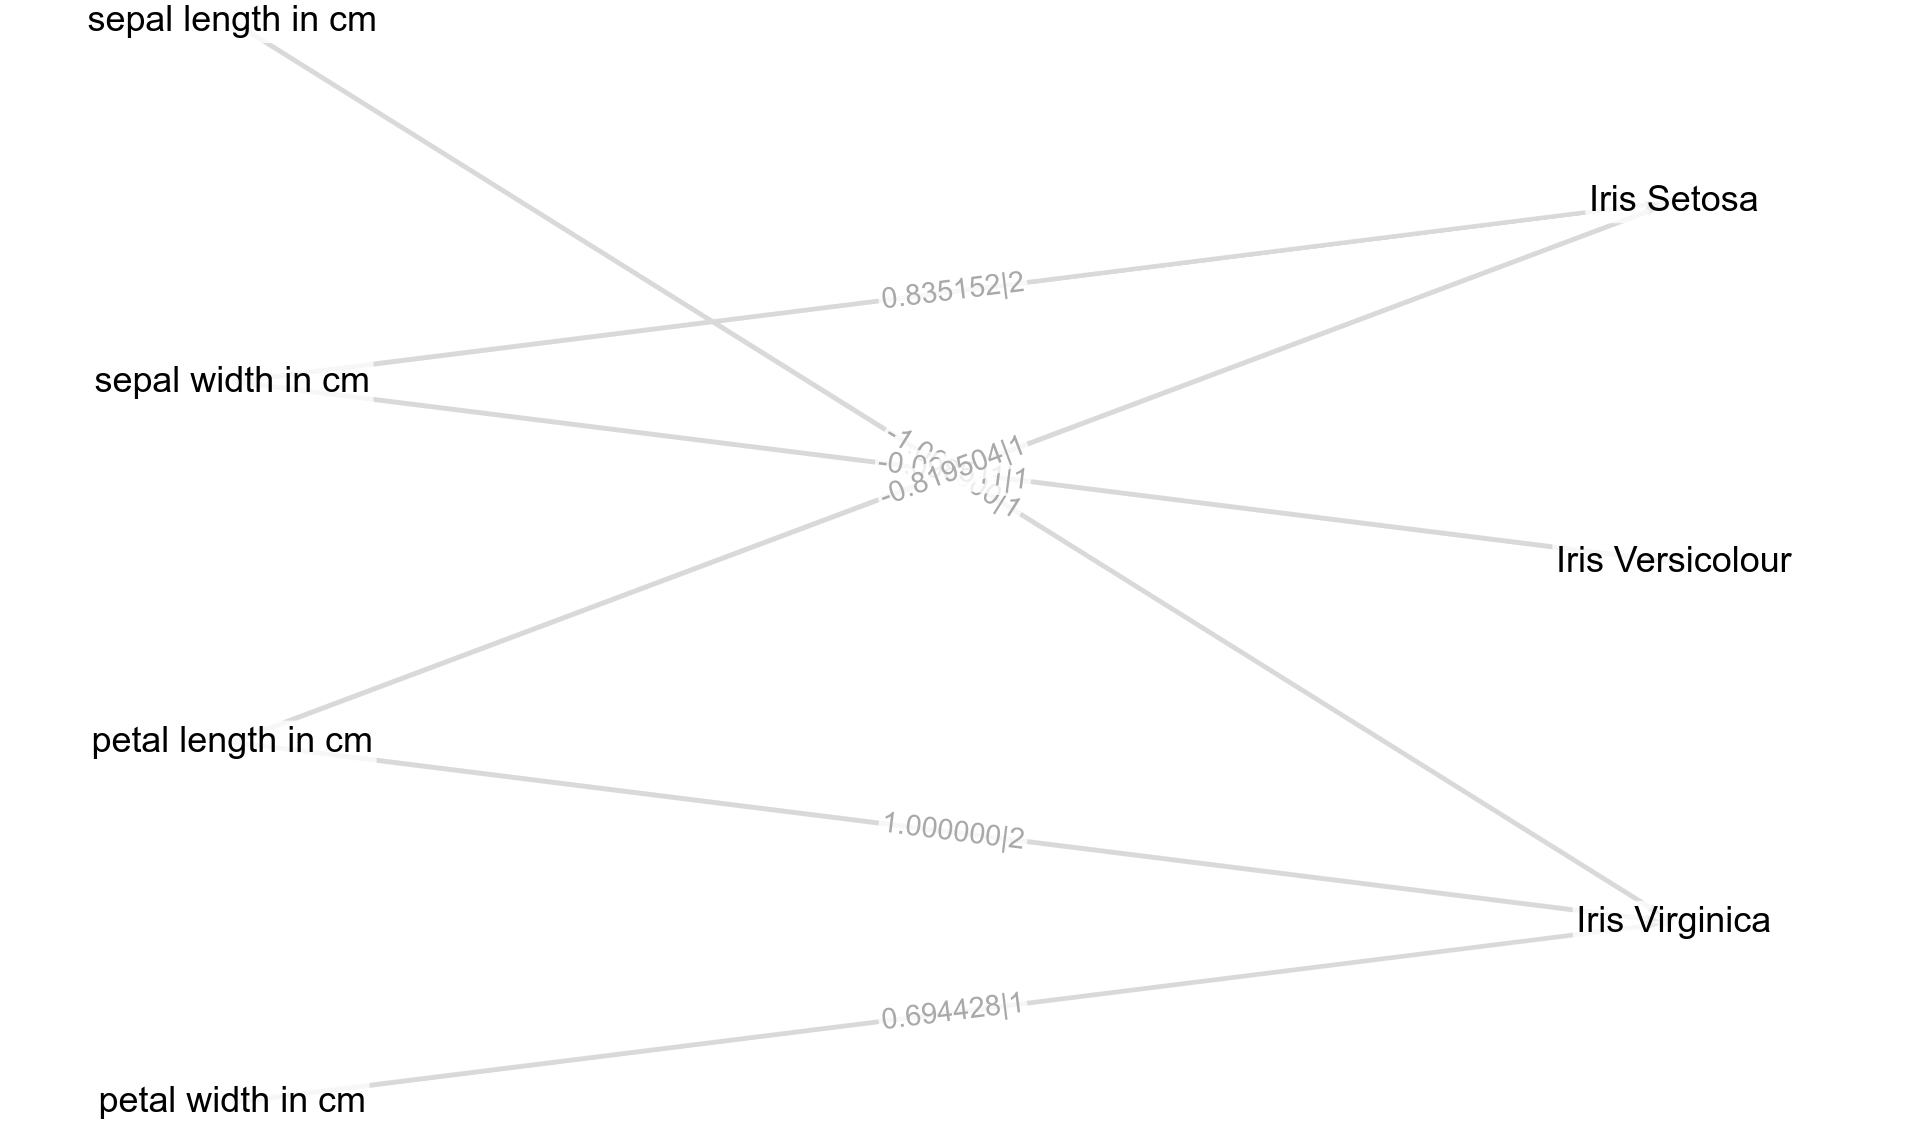
\includegraphics[width=13cm]{iris/2/mcc_g}
    \end{center}
    \caption{Vizualizacija agenta z največjim MCC drugega nabora. Vsebuje 6 povezav.}
    \label{fig:iris_mcc_2_g}
\end{figure}

\subsection{Tretji nabor}\label{subsec:dodatek-iris-tretji-nabor}
%%"/home/jure/CLionProjects/Neuroevolution/datasets/iris/iris.data" 200 15 30 3 true 0.1 100 true -0.001 -0.001 300 ACC
\begin{table}[H]
    \begin{center}
        \begin{tabular}{|| c | c c || c c ||}
            \hline
            \multirow{2}{*}{št. zagona} & \multicolumn{2}{c||}{točnost najboljšega agenta} & \multicolumn{2}{c||}{MCC najboljšega agenta} \\ \cline{2-5}
            & učna    & testna           & učna  & testna         \\
            \hline
            1        & 94.3\% & \textbf{97.8\%} & 0.972 & 0.906          \\
            \hline
            2        & 95.2\% & 84.4\%          & 0.986 & 0.936          \\
            \hline
            3        & 98.1\% & 95.6\%          & 0.972 & 0.839          \\
            \hline
            4        & 97.1\% & 93.3\%          & 0.958 & 0.936          \\
            \hline
            5        & 95.2\% & 93.3\%          & 0.972 & \textbf{0.967 (97.8\%)} \\
            \hline
            $\sigma$ & 0.014   & 0.046            & 0.009 & 0.043          \\
            \hline
        \end{tabular}
    \end{center}
    \caption{Rezultat tretjega nabora parametrov.}
    \label{tab:iris_result_3}
\end{table}

\begin{table}[H]
    \centering
    \begin{tabular}{||rcccc||}
        \hline
        razred           & Iris Setosa & Iris Versicolour & Iris Virginica & vsota \\ \hline
        ris Setosa       & 15          & 0                & 0              & 15    \\ \hline
        Iris Versicolour & 0           & 14               & 1              & 15    \\ \hline
        Iris Virginica   & 0           & 0                & 15             & 15    \\ \hline
        vsota            & 15          & 14               & 16             & 45    \\ \hline
    \end{tabular}
    \caption{Matrika zmot najbolj točnega agenta tretjega nabora.}
    \label{tab:iris_acc_3}
\end{table}

\begin{table}[H]
    \centering
    \begin{tabular}{||rcccc||}
        \hline
        razred           & Iris Setosa & Iris Versicolour & Iris Virginica & vsota \\ \hline
        ris Setosa       & 15          & 0                & 0              & 15    \\ \hline
        Iris Versicolour & 0           & 14               & 1              & 15    \\ \hline
        Iris Virginica   & 0           & 0                & 15             & 15    \\ \hline
        vsota            & 15          & 14               & 16             & 45    \\ \hline
    \end{tabular}
    \caption{Matrika zmot agenta z največjim MCC tretjega nabora.}
    \label{tab:iris_mcc_3}
\end{table}

\begin{figure}[H]
    \begin{center}
        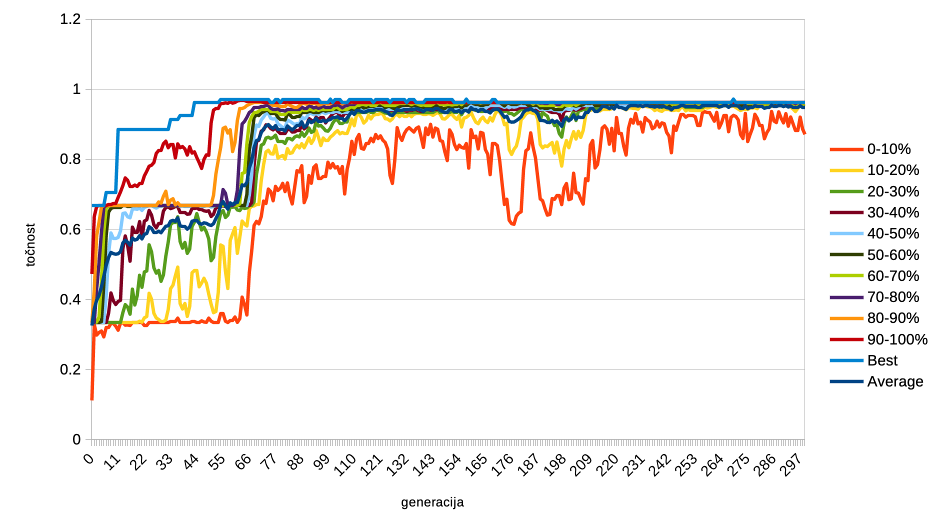
\includegraphics[width=13cm]{iris/3/acc}
    \end{center}
    \caption{Graf točnosti populacije najboljšega agenta tretjega nabora skozi generacije.}
    \label{fig:iris_acc_3}
\end{figure}

\begin{figure}[H]
    \begin{center}
        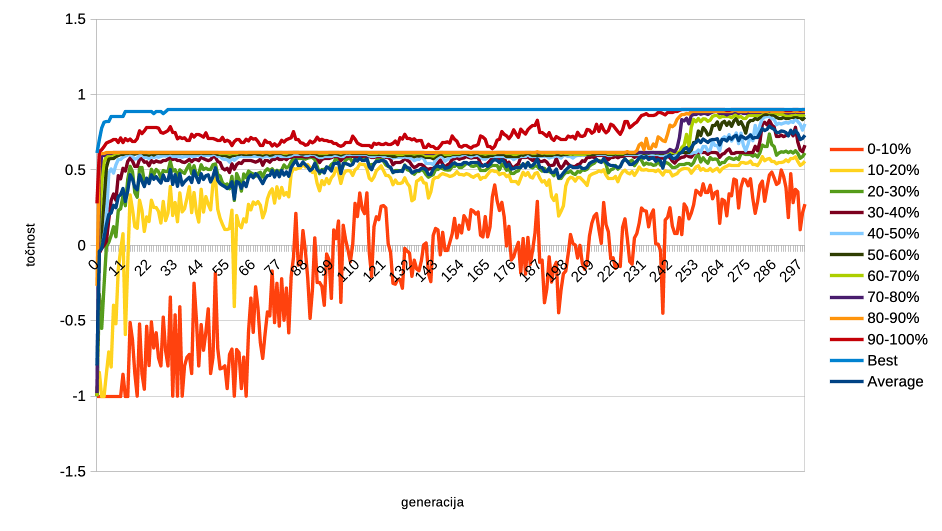
\includegraphics[width=13cm]{iris/3/mcc}
    \end{center}
    \caption{Graf MCC populacije najboljšega agenta tretjega nabora skozi generacije.}
    \label{fig:iris_mcc_3}
\end{figure}

\begin{figure}[H]
    \begin{center}
        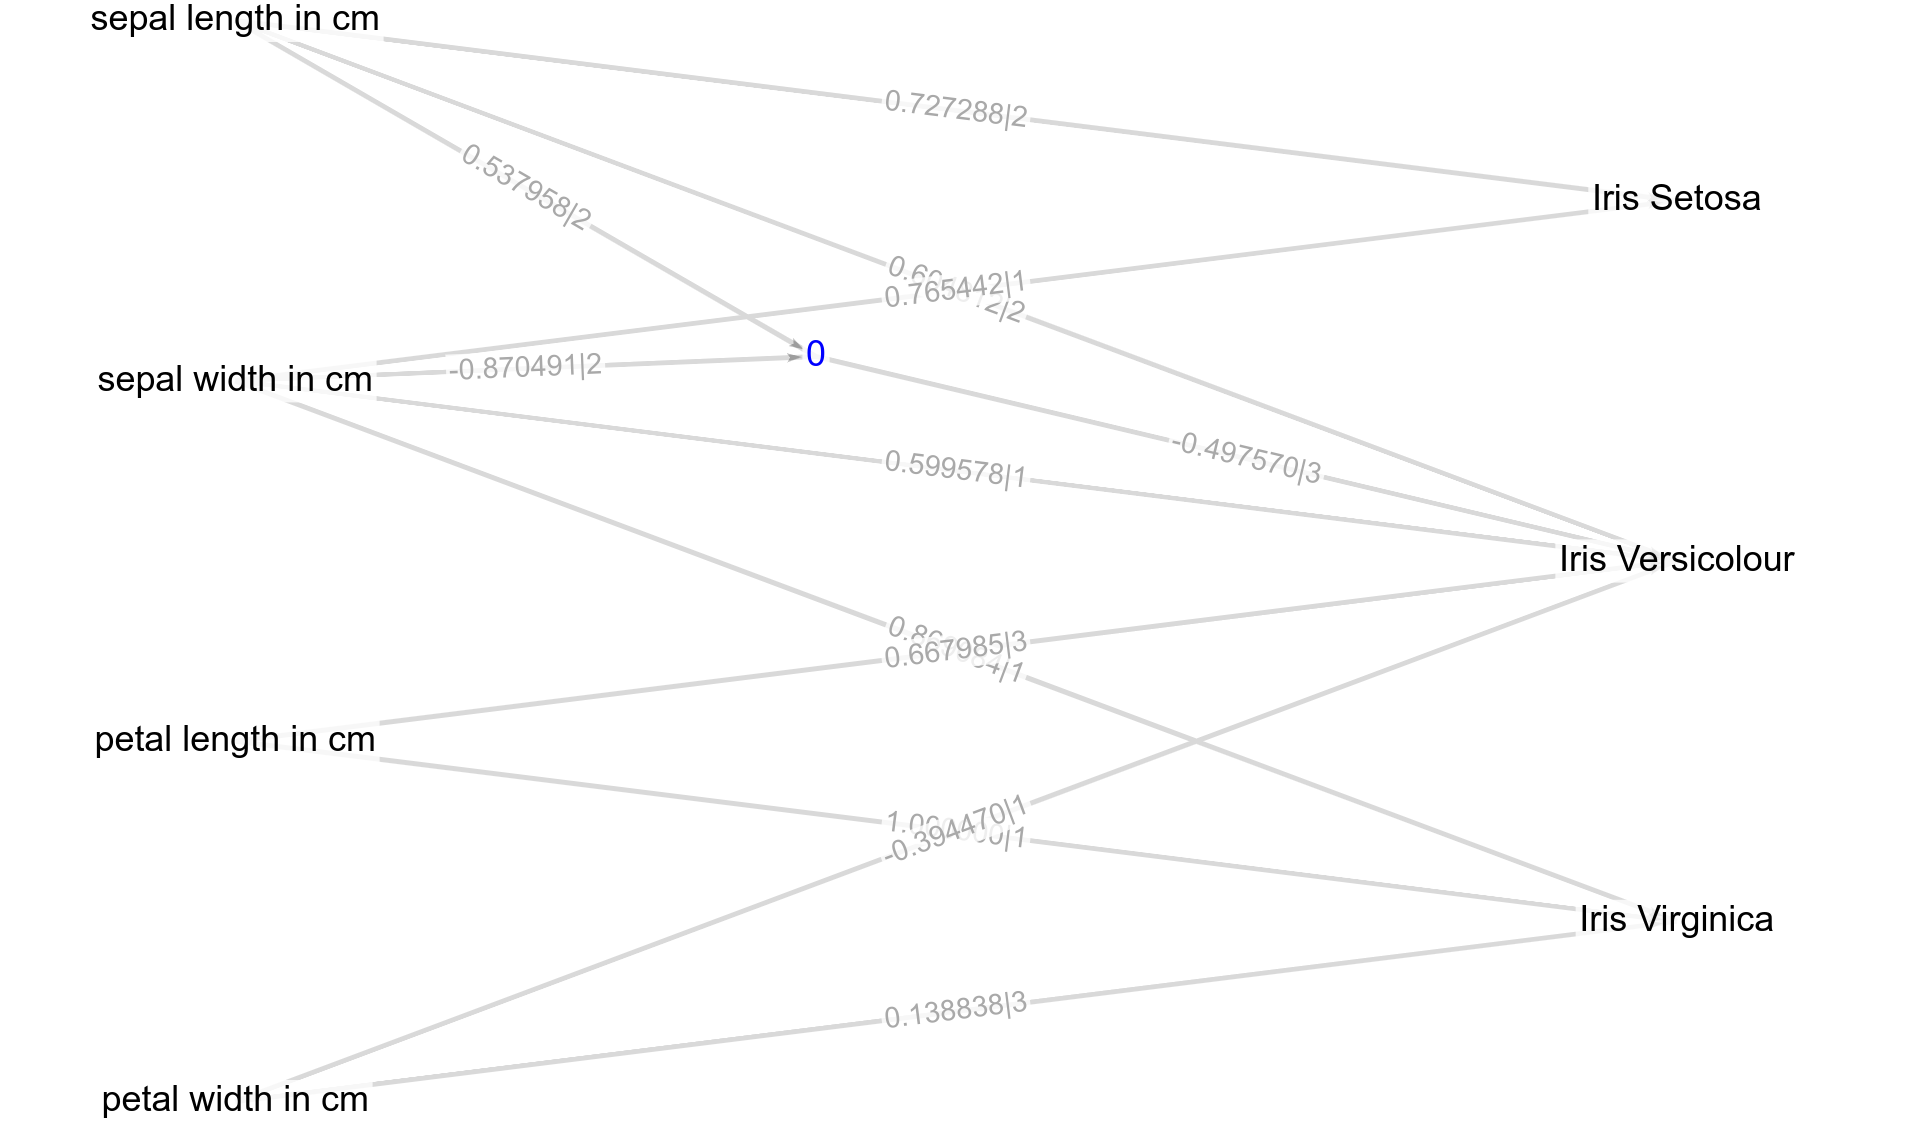
\includegraphics[width=13cm]{iris/3/acc_g}
    \end{center}
    \caption{Vizualizacija najbolj točnega agenta tretjega nabora. Vsebuje 6 povezav.}
    \label{fig:iris_acc_3_g}
\end{figure}

\begin{figure}[H]
    \begin{center}
        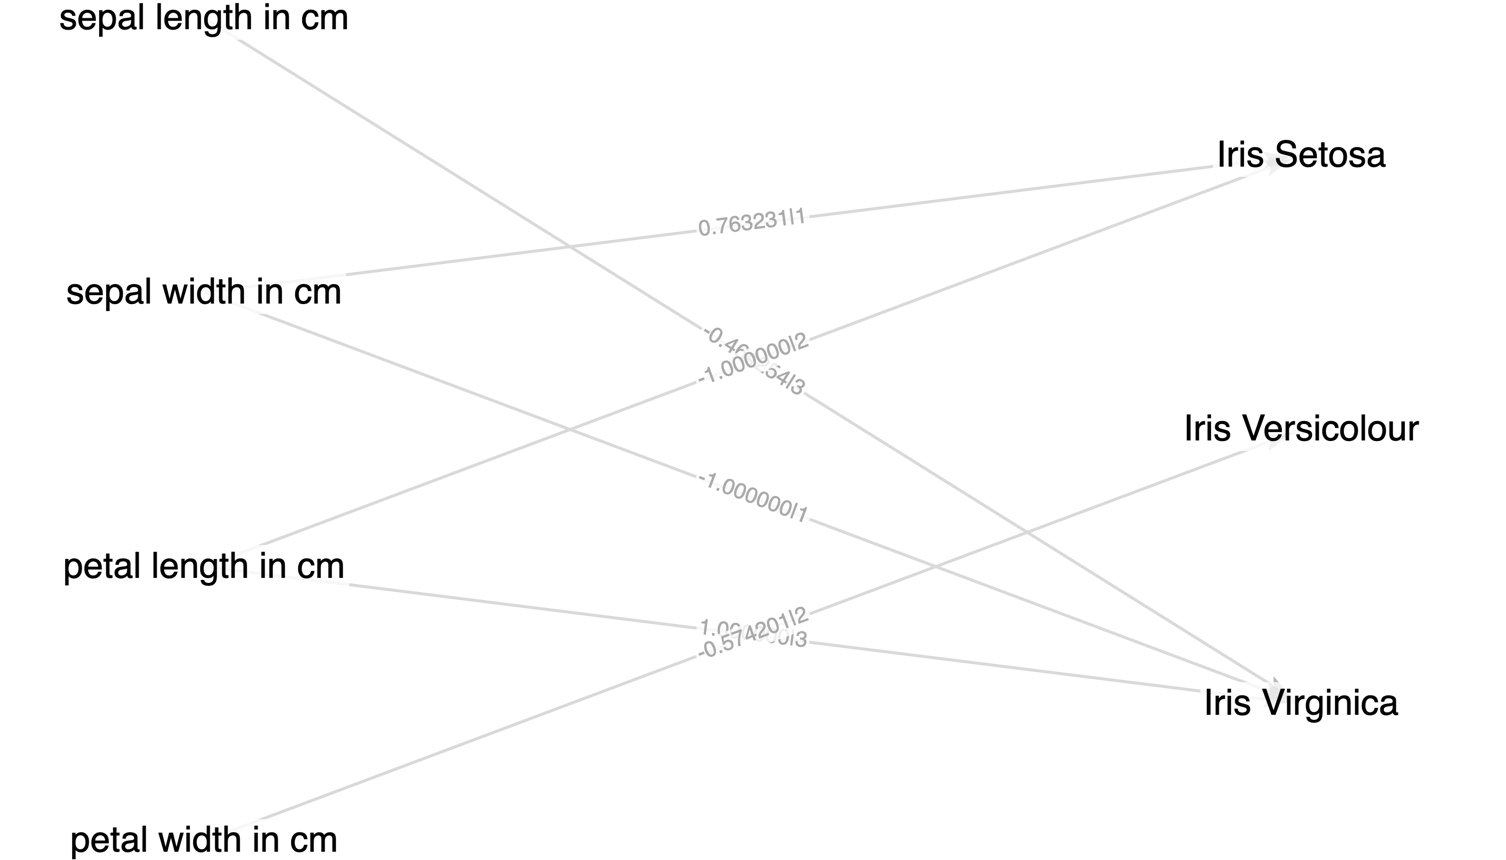
\includegraphics[width=13cm]{iris/3/mcc_g}
    \end{center}
    \caption{Vizualizacija agenta z največjim MCC drugega nabora. Vsebuje 6 povezav.}
    \label{fig:iris_mcc_3_g}
\end{figure}